\documentclass[10pt,oneside,a4paper]{article}

\bibliographystyle{naturemag}

\usepackage{graphicx}
\usepackage{grffile}
\usepackage{subfigure}
\usepackage{color} 
\usepackage{parskip}
\usepackage{float}
\usepackage{microtype}
\usepackage{times}
\usepackage{url}
\usepackage{hyperref}
\usepackage{longtable}
\usepackage[margin=0.65in]{geometry}
\usepackage{array}
\usepackage[labelfont=bf,labelsep=period,font=small,skip=5pt,font=scriptsize]{caption}
\usepackage{amsmath}
\usepackage{authblk}
\usepackage{ulem}
\usepackage{booktabs}
\usepackage{lineno}
\usepackage[outercaption]{sidecap} 

\newcommand\tab[1][1cm]{\hspace*{#1}}
\renewcommand{\arraystretch}{0.5}
\normalem
% To rename the figures' label:
\makeatletter 
\renewcommand{\thefigure}{S\@arabic\c@figure}
\makeatother
% To switch off page numbering:
\pagenumbering{gobble}
% \linenumbers

\begin{document}
  %\section*{Supplementary Information}

\begin{figure}[H]
    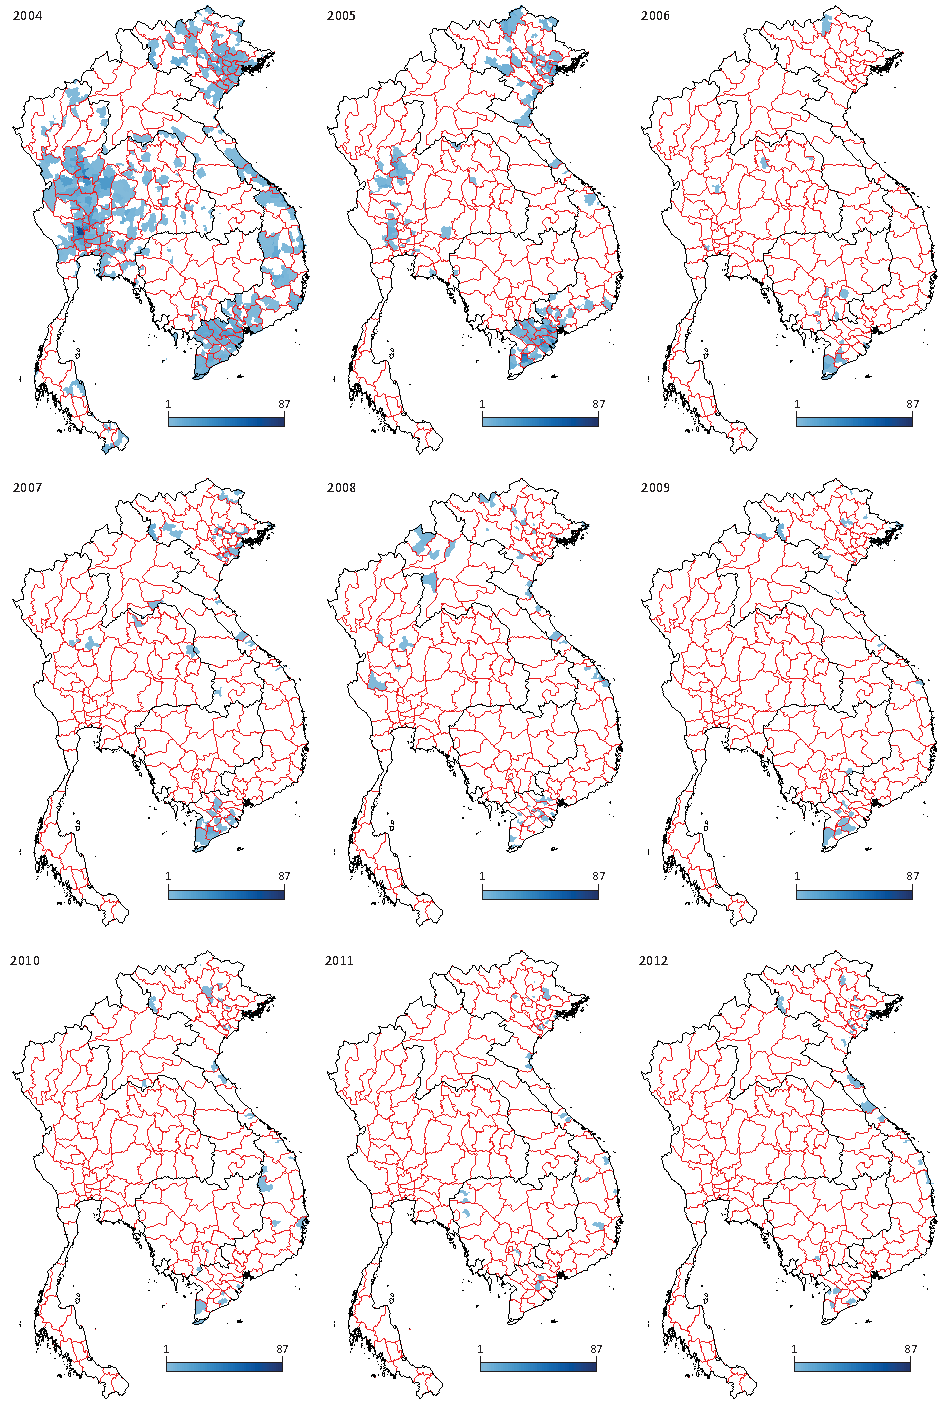
\includegraphics[width=1\textwidth]{Figure_S1.pdf}
	\caption{\scriptsize{\textbf{XXXX.}
XXXX.}}
\label{FigureS1}
\end{figure}

\begin{figure}[H]
    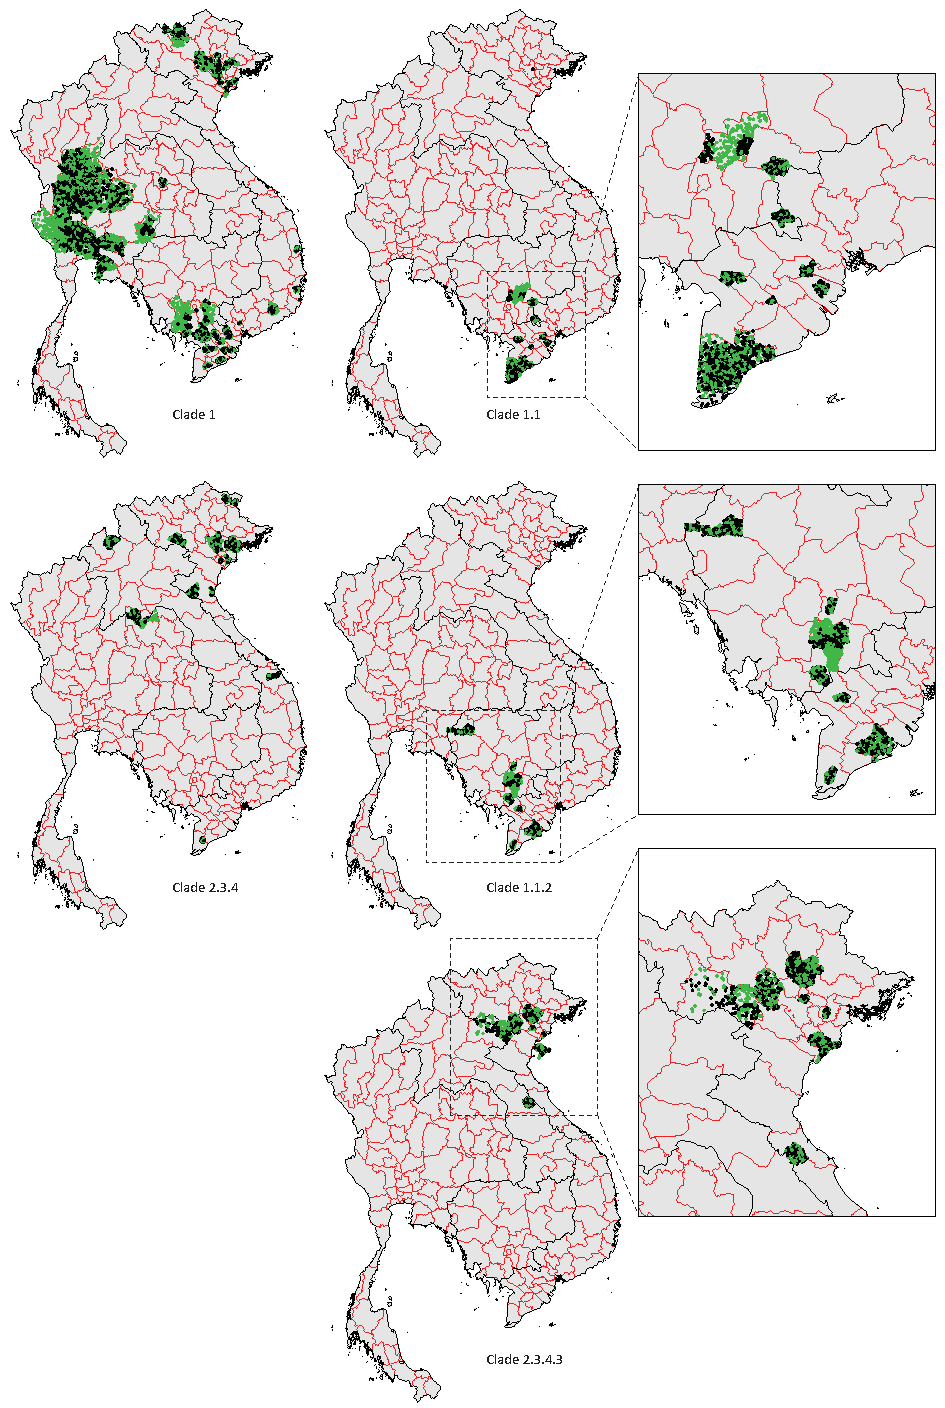
\includegraphics[width=1\textwidth]{Figure_S2.pdf}
	\caption{\scriptsize{\textbf{XXXX.}
XXXX.}}
\label{FigureS2}
\end{figure}

\begin{SCfigure}[][h]
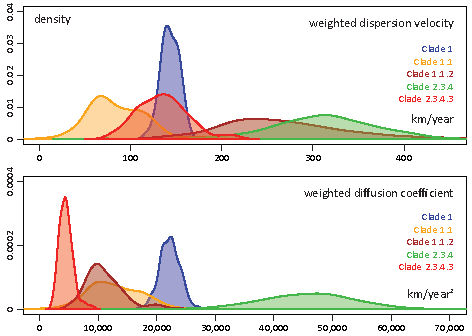
\includegraphics[width=0.5\textwidth]{Figure_S3.pdf}
	\caption{\scriptsize{\textbf{XXXX.}
XXXX.}}
\label{FigureS3}
\end{SCfigure}

\bigskip\bigskip

\begin{SCfigure}[][h]
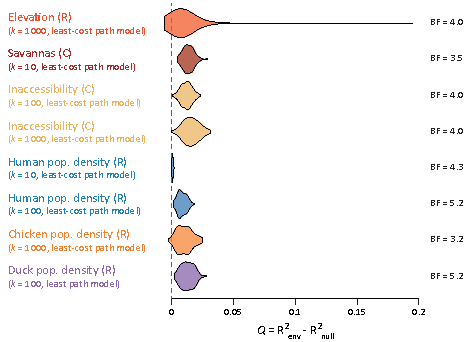
\includegraphics[width=0.5\textwidth]{Figure_S4.pdf}
	\caption{\scriptsize{\textbf{XXXX.}
XXXX.}}
\label{FigureS4}
\end{SCfigure}

\end{document}
